\lecture{Лекция 3}{lec3}
\subtitle{Лекция 3 --- Теория множеств}

\frame[plain]
{\titlepage}	% Титульный слайд


\begin{frame}
\frametitle{Теория множеств}

\begin{center}

\Huge
Понятие множества
	
\end{center}


\end{frame}

\begin{frame}
\frametitle{Множество}

\emph{Множества} состоят из \emph{элементов}.

Запись $x\hm\in M$ означает, что $x$~является элементом множества~$M$.

Есть некоторый объект. Когда он попадает в множество, то становится его \alert{элементом}.

\begin{block}{Пример}
$$ M=\{1,2,3\}$$
\end{block}

\end{frame}
\begin{frame}
\frametitle{Множество}
Предполагается существование некоторой универсальной совокупности объектов, из которой можно хотя бы мысленно выбирать объекты, чтобы затем составлять из них множества или рассматривать, принадлежат ли они данному множеству или нет. 

На природу объектов не накладывается никаких ограничений (в частности, объекты сами могут быть
множествами), за исключением того, что объекты должны быть определенными и различными. 

\end{frame}

\begin{frame}
\frametitle{Множество}
Множество само может рассматриваться как единый объект и в качестве такового входить в состав какого-нибудь другого множества.
\end{frame}

\begin{frame}
\frametitle{Множество}
Для любых двух объектов, рассматриваемых
в качестве элементов некоторого множества, должна иметься возможность определить, различны они или нет. 

Множества определяются своими элементами --- объектами, из которых они состоят. 

Два множества равны тогда и только тогда, кода они состоят из одних и тех же элементов. 
\end{frame}

\begin{frame}
\frametitle{Виды множеств}

\begin{itemize}
	\item Конечное множество: $M=\{1,2,3\}$
	\item Бесконечное множество: $M=\{1,2,3,\ldots,n,\ldots\}$. Натуральные числа
	\item Пустое множество: не содержит элементов. Обозначается $\varnothing$
\end{itemize}
\end{frame}


\begin{frame}
\frametitle{Подмножество}

Говорят, что множество~$A$ является \emph{подмножеством}
множества~$B$ (запись: $A\hm\subset B$),
если все элементы~$A$ являются элементами~$B$.

Если $A$ подмножество~$B$, не равное всему~$B$, то~$A$~называют
\emph{собственным} подмножеством~$B$


\end{frame}

\begin{frame}
\frametitle{Количество подмножеств}

Если множество содержит $n$ элементов, то число подмножеств равно $2^n$.

Закодируем элементы, входящие в подмножество битовой цепочкой: 0 не берем элемент, 1 берем элемент.\\
Например для множества  $A=\{1,2,3,4 \}$ подмножество $B=\{2,4\}$ будет закодировано как 0101.

Соответственно количество подмножеств равно количеству чисел, которые можно закодировать с помощью $n$ бит.



\end{frame}

\begin{frame}
\frametitle{Пустое множество}

\emph{Пустое} 
множество~$\varnothing$ не содержит ни одного
элемента и является подмножеством любого множества.
\end{frame}


\begin{frame}
\frametitle{Равенство множеств}
Множества~$A$ и~$B$
\emph{равны} 
(запись: $A\hm=B$), если они
содержат одни и те же элементы (другими словами, если
$A\hm\subset B$ и~$B\hm\subset A$).

\end{frame}


\begin{frame}
\frametitle{Способы задания множеств}
\begin{enumerate}
	\item Перечислением элементов: $A=\{1,3, 100 \}$ 
	\item Описанием: Множество всех тигров России
	\item Правилом выбора элементов: $A=\{x|(x\in N)\; и\;(x \leq 5) \}$
\end{enumerate}

\end{frame}

\begin{frame}
\frametitle{Универсальное множество}

Множество, которое содержит все другие множества в качестве подмножеств называется \textbf{универсальным} множеством.

\end{frame}

\begin{frame}
\frametitle{Определить элементы множеств}

Пусть дано универсальное множество $U=\{1,2,3,4,5,6,7,8,9\}$.

\begin{enumerate}
	\item $A=\{x|x \leq 5\}$\pause
	\item $B=\{x|x\; -\; четное\}$\pause
	\item $C=\{x|3<x \leq 6\}$\pause
	\item $D=\{x|x$ делится на 3 $\}$\pause
	\item $E=\{x|x$ содержит 2 единицы в двоичном коде$\}$
\end{enumerate}

\end{frame}

\begin{frame}
\frametitle{Какие из следующих утверждений верны?}
\small
\begin{tabular}{llll}
1. $b\subset \{a,b\}$ \pause &	2. $b\in \{a,b\}$ \pause &	3. $\{b\} \subset \{a,b\}$ \pause&	4. $\{b\} \in \{a,b\}$ \pause\tabularnewline
 & & & \tabularnewline
5. $b\subset \{a,\{b\}\}$ \pause &	 6. $b\in \{a,\{b\}\}$\pause &	 7. $\{b\}\subset \{a,\{b\}\}$ \pause &	 8. $\{b\}\in \{a,\{b\}\}$\pause \tabularnewline
& & & \tabularnewline
 9. $\varnothing \in \{ \varnothing\}$ \pause& 10. $\varnothing \subset \{ \varnothing\}$ \pause & 11. $\varnothing \in \varnothing$	\pause & 12. $\varnothing \subset \varnothing$ \tabularnewline

\end{tabular}
\end{frame}

\begin{frame}
\frametitle{Сколько элементов в каждом из множеств?}

\begin{enumerate}
	\item $\{1\}$\pause
	\item $\{1,2,3\}$\pause
	\item $\{1,2,\{3\}\}$\pause
	\item $\{1,\{2,3\}\}$\pause
	\item $\{Вася\}$\pause
	\item $\{$Буквы слова <<крокодил>>$\}$
	
	
\end{enumerate}

\end{frame}

\begin{frame}
\frametitle{Сколько элементов в каждом из множеств?}

\begin{enumerate}
	\item $\{\{1\}\}$\pause
	\item $\{1,\{2\},3\}$\pause
	\item $\{\varnothing\}$\pause
	\item $\{\varnothing,\{\varnothing\}\}$\pause
	\item $\{x| x^2=-1\}$
	
	
\end{enumerate}

\end{frame}

\begin{frame}
\frametitle{Какие утверждения верны?}

Известно, что $A \subset B$ и $a \in A$.

\begin{enumerate}
	\item $a \notin B$\pause
	\item $a \in B$\pause
	\item $A\in B$\pause
	\item $a \in A \cup B $\pause
	\item $a \in A \cap B$\pause
	\item $\{a\} \subset A$\pause
	\item $\{a\} \subset B$
	
\end{enumerate}

\end{frame}


\begin{frame}
\frametitle{Теория множеств}

\begin{center}

\Huge
Операции над множествами
	
\end{center}


\end{frame}

\begin{frame}
\frametitle{Объединение}

\emph{Объединение}
$A\cup B$\index{$\cup$} состоит из элементов, которые принадлежат хотя
бы одному из множеств~$A$ и~$B$:
        $$
A \cup B = \{ x\mid x\in A \text{ или } x\in B\}.
        $$

\begin{center}
\begin{tikzpicture}
    \draw[filled] \firstcircle node {$A$}
                  \secondcircle node {$B$};
    \node[anchor=south] at (current bounding box.north) {$A \cup B$};
\end{tikzpicture}
\end{center}

\end{frame}


\begin{frame}
\frametitle{Пересечение}

\emph{Пересечение}\index{Пересечение множеств}\index{Множества!пересечение}
$A\hm\cap B$\index{$\cap$} двух множеств~$A$ и~$B$
состоит из элементов, которые принадлежат обоим множествам~$A$
и~$B$. 
        $$
A \cap B = \{ x\mid x\in A \text{ и } x\in B\}
        $$

\begin{center}
% Set A and B
\begin{tikzpicture}
    \begin{scope}
        \clip \firstcircle;
        \fill[filled] \secondcircle;
    \end{scope}
    \draw[outline] \firstcircle node {$A$};
    \draw[outline] \secondcircle node {$B$};
    \node[anchor=south] at (current bounding box.north) {$A \cap B$};
\end{tikzpicture}

\end{center}

\end{frame}


\begin{frame}
\frametitle{Разность}

\emph{Разность}
$A\setminus B$ состоит из элементов, которые принадлежат~$A$, но
не принадлежат~$B$:
        $$
A \setminus B = \{ x\mid x\in A \text{ и } x\notin B\}.
        $$

\begin{center}
% Set A and B
\begin{tikzpicture}
     \begin{scope}
        \clip \firstcircle;
        \draw[filled, even odd rule] \firstcircle node {$A$}
                                     \secondcircle;
    \end{scope}
    \draw[outline] \firstcircle
                   \secondcircle node {$B$};
    \node[anchor=south] at (current bounding box.north) {$A \setminus B$};
\end{tikzpicture}

\end{center}

\end{frame}

\begin{frame}
\frametitle{Симметрическая разность}

\emph{Симметрическая разность}\index{Множества!симметрическая разность}%
\index{Симметрическая разность множеств} $A\bigtriangleup B$%
\index{$\bigtriangleup$} состоит из
элементов, которые принадлежат ровно одному из множеств $A$
и~$B$:
        $$
A \bigtriangleup B =
 (A\setminus B)\cup (B\setminus A)=(A\cup B)\setminus (A\cap B).
        $$
				
\begin{center}
% Set A and B
\begin{tikzpicture}
      \draw[filled, even odd rule] \firstcircle node {$A$}
                                 \secondcircle node{$B$};
    \node[anchor=south] at (current bounding box.north) {$A \bigtriangleup B$};
\end{tikzpicture}

\end{center}

\end{frame}

\begin{frame}
\frametitle{Дополнение}

Если множество
$B$~является подмножеством
множества~$A$, разность $A\setminus B$
называют также \emph{дополнением~$B$ до~$A$}\index{Дополнение множества}.

 $$
\overline{A} =  \{ x\mid x\notin A\}.
        $$
				
\begin{center}
% Set A and B
\begin{tikzpicture}
      \draw [filled, even odd rule] (-4.5,4) rectangle (4.5,0);
			\draw [fill=white] (0,2) circle (1.5);
\end{tikzpicture}

\end{center}

\end{frame}

\begin{frame}
\frametitle{Диаграммы Эйлера-Венна}

 $$
(A \cap C)\cup (B \cap C)
        $$
				
\begin{center}
% Set A and B
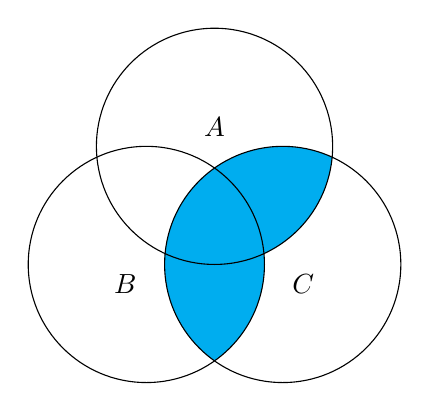
\begin{tikzpicture}
\def\firstcircle{(90:1.0cm) circle (1.5cm)}
  \def\secondcircle{(210:1.0cm) circle (1.5cm)}
  \def\thirdcircle{(330:1.0cm) circle (1.5cm)}
      \begin{scope}
    \clip \secondcircle;
    \fill[cyan] \thirdcircle;
      \end{scope}
      \begin{scope}
    \clip \firstcircle;
    \fill[cyan] \thirdcircle;
      \end{scope}
      \draw \firstcircle node[text=black,above] {$A$};
      \draw \secondcircle node [text=black,below left] {$B$};
      \draw \thirdcircle node [text=black,below right] {$C$};
\end{tikzpicture}

\end{center}

\end{frame}


\begin{frame}
\frametitle{Теория множеств}

\begin{center}

\Huge
Основные формулы
	
\end{center}


\end{frame}

\begin{frame}
\frametitle{Дополнение}

\begin{itemize}
	\item Коммутативность $ A \cup B= B\cup A$, $ A \cap B= B\cap A$, $ A \bigtriangleup B= B \bigtriangleup A$
	\item Ассоциативность $ A \cup (B\cup C)= (A \cup B)\cup C$, $  A \cap (B\cap C)= (A \cap B)\cap C$
	\item Дистрибутивность $ A \cap (B\cup C)= (A \cap B)\cup (A \cap C)$, $ A \cup (B\cap C)= (A \cup B)\cap (A \cup C)$
\end{itemize}

\end{frame}

\begin{frame}
\frametitle{Теория множеств}


\begin{center}

\Huge
Мощность множества	
\end{center}

\end{frame}

\begin{frame}
\frametitle{Мощность множества}

Число элементов в конечном
множестве~$A$ называют также его
\emph{мощностью}
и обозначают~$|A|$ (а также~$\#A$).

\end{frame}

\begin{frame}
\frametitle{Формула включений и исключений}

\begin{align*}
    |A\cup B|        & =|A|+|B|-|A\cap B|;\\
    |A\cup B \cup C| & =|A|+|B|+|C|-\\
                     &{}-|A\cap B|-|A\cap C|-|B\cap C|+\\
                     &{}+|A\cap B\cap C|;
\end{align*}

вообще $|A_1\cup\ldots\cup A_n|$ равно
        $$
      \sum_{i}|A_i| - \sum_{i<j}|A_i \cap A_j| +
      \sum_{i<j<k} |A_i \cap A_j \cap A_k| - \ldots
        $$


\end{frame}

\begin{frame}
\frametitle{Теория множеств: Задача}
В языке запросов поискового сервера для обозначения логической операции «ИЛИ» используется символ «|», а для логической операции «И» - символ «\&». В таблице приведены запросы и количество найденных по ним страниц некоторого сегмента сети Интернет.
\begin{tabular}{|c|c|}
\hline 
 Запрос &Найдено страниц (в тысячах) \tabularnewline
\hline 
Лебедь(A) \& (Рак (B) | Щука(C)) &  320 \tabularnewline
\hline 
Лебедь \& Рак & 200 \tabularnewline
\hline 
Лебедь \& Рак \& Щука & 50 \tabularnewline
\hline 
\end{tabular}

Какое количество страниц (в тысячах) будет найдено по запросу (Лебедь \& Щука)\\
Считается, что все запросы выполнялись практически одновременно, так что набор страниц, содержащих все искомые слова, не изменялся за время выполнения запросов.

\end{frame}

\begin{frame}
\frametitle{Теория множеств: Решение}
По формуле включений и исключений имеем:
 $$
|A \cap (B \cup C)|=|A\cap C| + |A \cap B| - |A \cap B \cap C|.
$$
 
Тогда искомое количество страниц:
$$
|A \cap C| = 320 - 200 + 50 = 170
$$
\end{frame}




